\section{Описание практической части}
\label{sec:Chapter4} \index{Chapter4}

\subsection{Описание программной реализации}

Для написания данной программы рассматривались 3 языка программирования: Ассемблер, С и С++. Ассемблер
практически сразу был исключен из рассмотрения в виду его крайне большой зависимости от конечной платформы.
Но следующий выбор уже не был таким очевидным, ведь С и С++ очень похожи. В конечном счёте выбор
был сделан в пользу C, т.к. он даёт больше контроля программисту над тем, что делает программа, и
над памятью, которая выделяется и используется в программе.

А в качестве инструмента параллельного запуска на всех узлах был выбран MPI стандарта 3.1 как
самый младший из наиболее часто установленных стандартов.

При запуске программа ничего не читает со стандартного ввода, а только анализирует аргументы командной
строки. Первый аргумент является обязательным и представляет из себя размер файла, который будет
записывать на диск. Второй и последующие аргументы является опциональными и должны представлять из себя
цифры от 1 до 6, таким образом указываются тесты, которые будут производиться. Если будет указан только
первый параметр, то будут запущены все тесты.

После работы главный процесс собирает все данные и выводит на стандартный вывод 12 чисел с плавающей
точкой, разделенные пробелом. Первые шесть цифр - это скорость записи файлов на диск (байт в секунду), а
последние 6 - это скорость чтения файлов с диска (байт в секунду).

В тестирующей программе был реализован следующий набор тестов:
\begin{description}
    \item[$\bullet$] Асинхронная коллективная запись в один файл
    \item[$\bullet$] Асинхронная не коллективная запись в один файл
    \item[$\bullet$] Синхронная коллективная запись в один файл
    \item[$\bullet$] Синхронная не коллективная запись в один файл
    \item[$\bullet$] Асинхронная не коллективная запись в один файл, но каждый процесс
    пишет в случайное место в файле
    \item[$\bullet$] Асинхронная не коллективная запись каждого процесса
    в свой собственный файл
\end{description}

Асинхронная запись означает, что данный процесс после того, как пошлёт запрос на запись,
может продолжать работать и выполнять какие-то вычисления, а не ожидать окончания записи в файл.

Коллективая запись означает, что перед записью все процессы синхронизируются и могут
оптимизировать запись данных в файл, например, переслать часть данных в другой процесс,
чтобы меньшее количество процессов производило запись в файл.

Первые 4 теста должны показывать примерно одинаковую производительность, они осуществляют тестирование производительности серверов хранения и параллельную запись с помощью MPI-IO.

Пятый тест производит нагрузочное тестирование серверов хранения, так как он получает очень
большое количество запросов на запись в случайные места диска, а это тратит намного больше ресурсов,
чем линейная запись в файл (как для записи на сервера хранения, так и для определения размеров
файла на сервере метаданных).

Шестой тест производит нагрузочное тестирование сервера метаданных и проводит замер скорости
чтения-записи на сервера хранения данных, потому что происходит создание очень большого количества различных файлов.

\subsection{Тесты проведённые на суперкомпьютере МВС-10П МП2}

\begin{figure}[h]
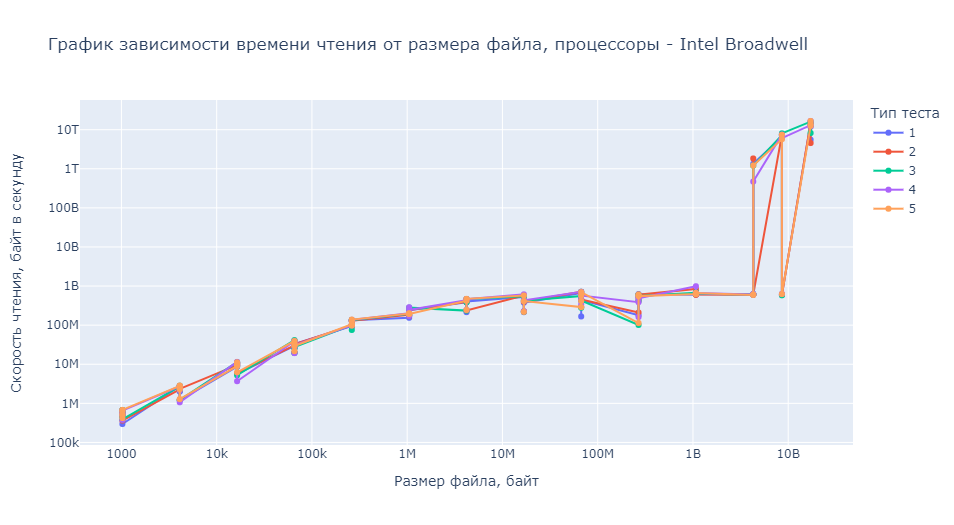
\includegraphics[height=9cm,keepaspectratio]{./test_graphs/read_broadwell.png}\\[0.1cm]
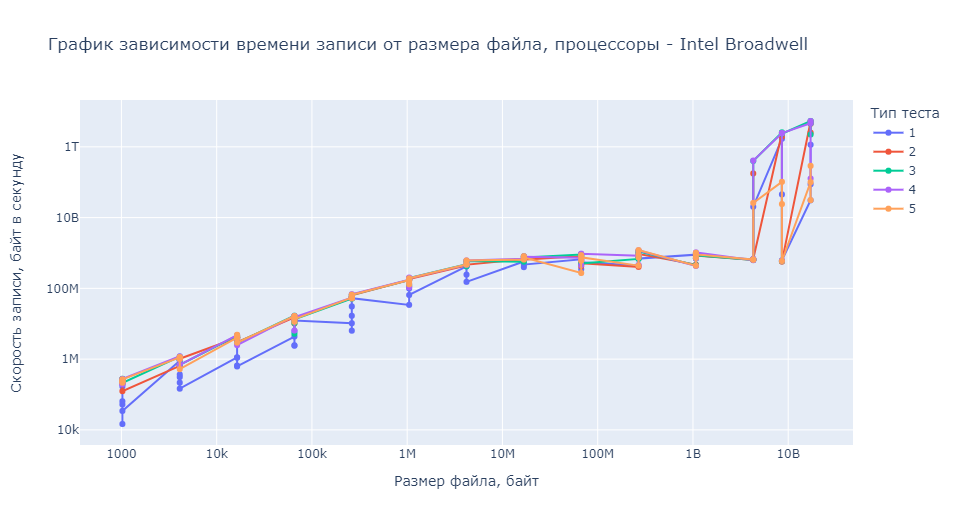
\includegraphics[height=9cm,keepaspectratio]{./test_graphs/write_broadwell.png}\\[0.1cm]
\caption{Тесты на разделе \textbf{Broadwell}}
\label{broadwell}
\end{figure}

\begin{figure}[h]
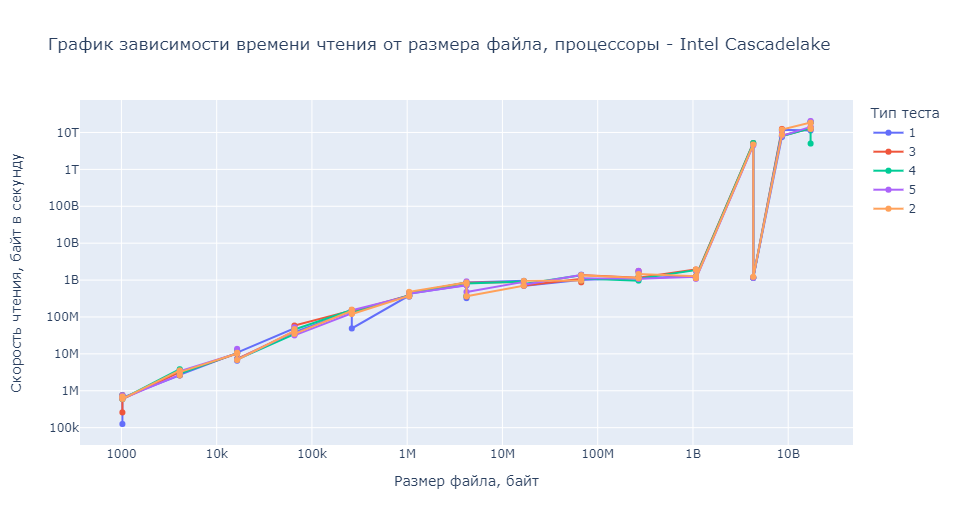
\includegraphics[height=9cm,keepaspectratio]{./test_graphs/read_cascadelake.png}\\[0.1cm]
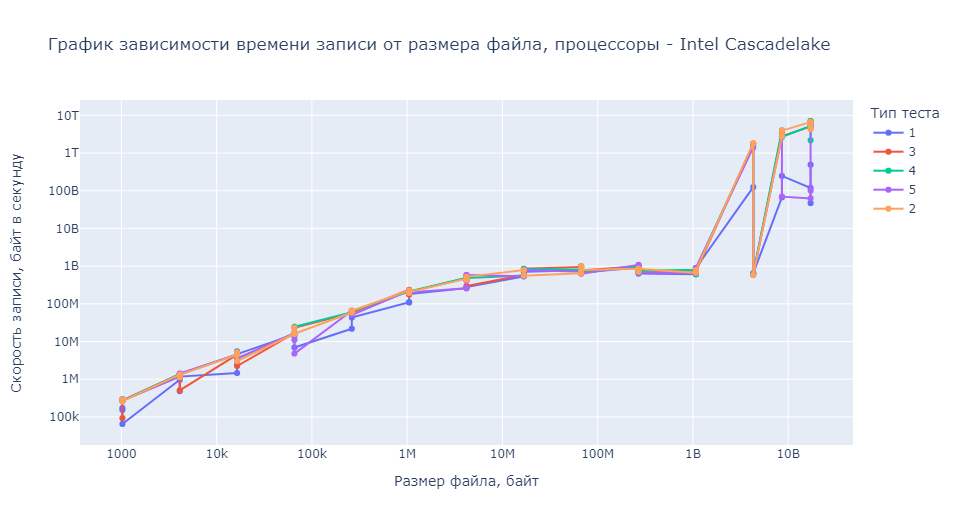
\includegraphics[height=9cm,keepaspectratio]{./test_graphs/write_cascadelake.png}\\[0.1cm]
\caption{Тесты на разделе \textbf{Cascade\_lake}}
\label{cascadelake}
\end{figure}

На графиках \ref{broadwell} можно увидеть зависимость скорости чтений и записи файлов. Замеры производительности были осуществлены на разделе кластера под названием \textbf{Broadwell}. Технические характеристики:
\begin{description}
    \item[$\bullet$] 136 вычислительных модулей на базе 16-ядерных процессоров Intel Xeon Broadwell
    \item[$\bullet$] Коммуникационная среда - Intel Omni-Path
    \item[$\bullet$] Каждый узел включает в себя 2 процессора Intel Xeon E5-2697Av4 и 128 Гб оперативной памяти
\end{description}


На графиках \ref{cascadelake} можно увидеть зависимость скорости чтений и записи файлов. Замеры производительности
были осуществлены на разделе кластера под названием \textbf{Cascade\_lake}. Технические характеристики:
\begin{description}
    \item[$\bullet$] 47 вычислительных модулей на базе 24-ядерных процессоров Intel Xeon Cascade Lake
    \item[$\bullet$] Коммуникационная среда - Intel Omni-Path
    \item[$\bullet$] Каждый узел включает в себя 2 процессора Intel Xeon Platinum 8268 2.90 GHz и 192 Гб
    оперативной памяти
\end{description}

Ввиду того, что на сервере присутствует дисковая квота в 17 гигабайт, запустить тест под номер 6 для сбора достаточной статистики оказалось невозможно, поэтому в данных присутствуют тесты с 1 по 5.

Если взглянуть на графики, то можно заметить, что для теста с одним размером файла было сделано несколько
запусков, при это скорость чтения-записи на этих тестах не отклоняется больше чем на 50\% от среднего
значения. Это значит, что lustre работает исправно и хорошо воспринимает параллельные потоки данных и
исправно функционирует, позволяя записывать данные параллельно.

Причём, как видно из графика, при увеличении размера файла, также растёт и скорость записи файла на диск,
это связано с тем, что растёт процент полезной нагрузки на сеть, ведь при записи или чтении файла MPI
сначала устанавливает связь со всеми процессами, они обмениваются между собой служебной информацией и
только после этого начинает переделывать сам файл для записи на диск. Также это можно связать с тем, что
файл начинает разбиваться на большее количество частей при записи на дисковое пространство. Этот процесс
называется File Striping - распределение одного файла между несколькими физическими или логическими
местами хранения файлов путём разбиения его на несколько частей. И как видно из графика, когда размер
файла достиг нескольких гигабайт распределение файла между несколькими серверами хранения стало более
агрессивное, что позволило ещё больше расспараллелить чтение-запись файла на диск, а как следствие
повысило скорость операций ввода-вывода.

